\documentclass[pdflatex,sn-mathphys-num]{sn-jnl}
\usepackage{graphicx,amsmath,amssymb,booktabs,tabularx,url,xurl,microtype,etoolbox,placeins,flafter,needspace}
\raggedbottom
\AtBeginDocument{\let\burl\url}
\AtBeginEnvironment{thebibliography}{\interlinepenalty=10000}
\makeatletter
% Keep the structured abstract together using the publisher's type sizes.
\patchcmd{\@maketitle}{\vskip21pt}{\vskip0pt}{}{\errmessage{Title spacing patch failed}}
\patchcmd{\@maketitle}{\vskip20pt}{\vskip0pt}{}{\errmessage{Article-title spacing patch failed}}
\patchcmd{\@maketitle}{\vskip20pt}{\vskip4pt}{}{\errmessage{Author spacing patch failed}}
\patchcmd{\abstracthead}{-22pt}{-8pt}{}{\errmessage{Abstract spacing patch failed}}
\patchcmd{\@maketitle}{\vskip24pt}{\vskip0pt}{}{\errmessage{Address spacing patch failed}}
\patchcmd{\@maketitle}{\vskip24pt}{\vskip0pt}{}{\errmessage{Email spacing patch failed}}
\def\ps@paper{\let\@oddhead\@empty\let\@evenhead\@empty
  \def\@oddfoot{\hfil\thepage\hfil}\let\@evenfoot\@oddfoot}
\let\ps@titlepage\ps@paper
\let\ps@headings\ps@paper
\makeatother
\pagestyle{paper}
% All numerical claims are expanded into generated fragments.

\begin{document}
\title[Crowd-label supervision for selective FER]{Evaluating Crowd-Label Supervision for Selective Facial-Expression Recognition}
\author[1]{\fnm{Gunjan Kumar} \sur{Mishra}}\email{mgunjan67@gmail.com}
\author[2]{\fnm{Bijaya} \sur{Ghimire}}\email{vijay.gh74@gmail.com}
\author*[3]{\fnm{Badri Raj} \sur{Lamichhane}}\email{d6622300231@g.siit.tu.ac.th}
\author[4]{\fnm{Alan} \sur{Shah}}\email{shahalan0202@gmail.com}
\affil[1]{\orgname{WorldQuant University}, \orgaddress{\city{Washington, D.C.}, \country{United States}}}
\affil[2]{\orgdiv{Department of Electronics and Computer Engineering}, \orgname{Institute of Engineering, Paschimanchal Campus}, \orgaddress{\city{Pokhara}, \country{Nepal}}}
\affil*[3]{\orgdiv{School of Information, Computer and Communication Technology}, \orgname{Sirindhorn International Institute of Technology, Thammasat University}, \orgaddress{\city{Pathum Thani}, \country{Thailand}}}
\affil[4]{\orgname{Herald College Kathmandu}, \orgaddress{\city{Kathmandu}, \country{Nepal}}}
\abstract{\noindent\textbf{Purpose:} Training on facial-expression vote distributions may improve distributional agreement without improving confidence-selected category predictions. We examine how that distinction depends on target probability values, tied maxima, accepted images and output vocabulary.
\par\smallskip
\noindent\textbf{Methods:} An adaptive within-source study on FER2013/FER+ comprised 24 original Swin-T/ResNet-18 runs and twelve additional Swin-T runs, with three paired seeds per condition. Soft retained vote proportions; Uniform kept one dominant probability and flattened the remainder, whereas Tie-Uniform preserved all tied maxima. A permutation preserved each target's probability multiset. Seven- and eight-expression classifiers were scored against all ten annotation categories. The primary reporting point accepted each model's 80\% most confident images. Analyses included fixed-image comparisons, checkpoint rules and confidence scores. Frozen original models were evaluated on 1,440 RAVDESS clips.
\par\smallskip
\noindent\textbf{Results:} Distance-selected seven-output Soft reduced disagreement by 0.79 percentage points relative to the entropy-preserving permutation. With eight outputs, Soft achieved 23.74\% disagreement versus 24.58\% for Uniform and 23.79\% for Tie-Uniform. The Soft-minus-Tie-Uniform difference was $-0.05$ points, with a conditional 95\% interval of $[-0.31,+0.21]$, and reversed under alternative rankings. Soft had lower squared distance in every matched softening-control comparison, but the original selective advantage did not persist across backbones. External transfer was poor and sensitive to aggregation and annotation reference.
\par\smallskip
\noindent\textbf{Conclusion:} The measured benefit of crowd-distribution supervision depends on the control and selection policy. Better distributional agreement does not establish a general advantage in selective categorical prediction.
}
\keywords{facial-expression recognition, crowd annotations, selective prediction, label distributions, supported vote mass, confidence calibration}
\maketitle

\section{Introduction}
Facial-expression recognition (FER) often assigns one category to an image, although annotators may disagree. FER+ retains this variation through multiple responses for FER2013 images \cite{goodfellow2013fer,barsoum2016ferplus}. Training on those distributions can improve agreement with human response frequencies without improving categorical decisions \cite{washington2021crowdsourcing}. Likewise, soft-label training does not necessarily improve selective prediction, in which a model withholds its less confident decisions \cite{khurana2024crowd,xia2025smoothing}. These distinctions are established; our question is what a controlled FER comparison adds to their interpretation.

Three choices complicate that comparison. First, replacing a hard target with a vote distribution changes its largest probability, treatment of tied maxima, and minority-category allocation together. A hard--soft difference cannot attribute the result to one of these changes. Second, models at equal coverage---the accepted fraction of images---may accept different images. Their reported disagreement combines category choices with the composition of those sets. Third, annotations can include categories absent from the model. Removing those votes changes the scoring reference and hides part of the disagreement.

We examine these choices using matched training targets, cross-evaluation on identical accepted images, and complete-vocabulary scoring. The original primary follow-up compares seven-output empirical vote targets (Soft) with a control retaining the largest target probability but spreading the remainder uniformly (Uniform). Tie-preserving controls address alternative handling of tied maxima. Initialization, images, weights, order, augmentation and optimization remain matched within each backbone and seed. The controls preserve specified properties rather than all aspects of the targets: Uniform also changes entropy and aggregate class proportions.

The study addresses three questions:
\begin{enumerate}
\item \textbf{Target information:} What selective advantage remains after controlling dominant target probabilities and ties, and after preserving each target's probability values while disrupting minority-category identities?
\item \textbf{Evaluation choice:} How does predictor ordering depend on accepted images and on whether the model includes seven or eight expression outputs?
\item \textbf{Robustness:} Which findings persist across tested backbones, confidence rankings, checkpoints, calibration transfer and external clips?
\end{enumerate}

Our contribution is an empirical comparison of these dependencies, rather than a new architecture or rejection algorithm. The original seven-output Swin-T comparison uses three paired seeds at 80\% coverage. Secondary analyses examine ResNet-18, fixed-epoch checkpoints and alternative confidence scores; follow-up controls test minority-category allocation and an eight-expression vocabulary. Together, the phases contain 36 training runs and 81 named checkpoint-rule states, not necessarily distinct weight sets. They are adaptive and reuse one image source, with each new comparison specified before its own outcomes. Frozen evaluation on 1,440 RAVDESS clips \cite{livingstone2018ravdess} assesses a different population and prediction unit, providing a transfer test rather than independent static-image confirmation.

A local messaging preview motivated the initial seven-category model. Related systems use text-based emotion notifications, facial and textual signals, or expression-informed emoji suggestions \cite{wang2016emotionpush,chong2019emochat,liu2019selfawareness}. Such cues do not establish a person's internal emotion or intention \cite{barrett2019emotions}. We retain the implementation as a supplementary artifact; the research evidence concerns annotation-based recognition and selection.


\section{Related work}
FER+ established distribution-based supervision for multiple annotations of FER2013 images \cite{barsoum2016ferplus}. Washington et al. compared hard and soft targets on CAFE and showed that categorical performance and agreement with response distributions can favor different models \cite{washington2021crowdsourcing}. Other FER methods use disagreement through weighting and relabeling, uncertainty-aware target construction, or soft-label video augmentation \cite{wang2020scn,le2023uncertainty,kawamura2024midas}. We retain the observed votes and compare their training representations under matched conditions, rather than benchmark the additional mechanisms of those methods.

Selective classification trades accepted coverage against prediction risk \cite{geifman2017selective}; SelectiveNet jointly learns prediction and rejection \cite{geifman2019selectivenet}. Crowd-Calibrator estimates annotator distributions to inform rejection in subjective language tasks \cite{khurana2024crowd}. In its hate-speech comparison, soft-label models improve soft and calibration measures without corresponding categorical gains, whereas soft-label MaxProb performs worse on AUC/AUROC selection measures. Thus, disagreement between distributional and selective outcomes is not a new general finding. Our FER evaluation asks what remains after matching dominant target probabilities and ties, holding accepted images fixed, and accounting for the complete annotation vocabulary. We do not implement its learned crowd estimator or claim directly comparable benchmark scores.

Xia et al. show that conventional label smoothing can worsen selective classification by changing the ranking of correct and incorrect predictions, and examine post hoc logit normalization \cite{xia2025smoothing}. Our Uniform control instead uses image-dependent dominant probabilities and our loss scores disagreement with empirical votes, rather than binary correctness. Nevertheless, the ranking explanation is directly relevant. We therefore examine probability-based scores and a normalization sensitivity without retraining the existing models; these analyses assess ranking dependence rather than establish a new selector.

Calibration against a majority label also differs from agreement with annotator distributions. Baan et al. demonstrate this distinction and develop measures of human-judgment distribution properties \cite{baan2022calibration}; Guo et al. examine conventional confidence calibration \cite{guo2017calibration}. We report distributional distance, selected categorical disagreement and achieved calibration-transfer risk separately. Lower squared distance is not interpreted as a deployment risk guarantee.

The backbones and channel gates use established Swin, ResNet and squeeze-and-excitation designs \cite{liu2021swin,he2016resnet,hu2018senet}. Vats and Chadha describe Swin with squeeze-and-excitation for FER (unpublished preprint, 2023; \href{https://arxiv.org/abs/2301.10906}{arXiv:2301.10906}). Recent unpublished preprints examine ambiguity-aware calibration (Tao et al., 2026; \href{https://arxiv.org/abs/2603.22879}{arXiv:2603.22879}), dynamic disagreement prediction (Wang et al., 2026; \href{https://arxiv.org/abs/2609.17130}{arXiv:2609.17130}), and routing between ambiguity and distribution shift (Inoshita and Ueno, 2026; \href{https://arxiv.org/abs/2606.22725}{arXiv:2606.22725}). These related methods are not implemented baselines; their results do not validate ours. Our contribution concerns controlled target comparisons and their interpretation, with no architecture or rejection-method novelty claimed.


\section{Methods}
\subsection{Study design and analysis hierarchy}
We compare training targets while matching architecture, initialization, image order, augmentation and optimization within each backbone and seed. The original four adaptive phases contain 24 runs and 48 retained validation-selected or epoch-12 states (Table~\ref{tab:phases}). Initial Hard/Soft results informed the Uniform/Tie-hard follow-up, followed by Tie-Uniform and ResNet-18 checks. Each phase was specified before its own training and calibration/test outcomes, but earlier PrivateTest results were known. These phases therefore provide adaptive within-source evidence.

The 80\% coverage endpoint was fixed in the original Hard/Soft protocol. The later Soft-minus-Uniform protocol inherited this reporting point and designated that contrast primary before its new outcomes. It was not chosen to maximize the observed follow-up effect and is not asserted to be an optimal operating point; other coverages are sensitivities. Distribution-distance summaries, confidence-score analyses and external diagnostics have the secondary or exploratory roles stated below. Follow-up target and vocabulary tests were specified after reviewing these earlier results and frozen before their own outcomes; they do not create an untouched confirmatory test.

The RAVDESS plan was frozen locally before external model outcomes, after internal findings and annotation summaries were known. A retained pre-analysis amendment corrected swapped disgust/surprise response indices against source descriptors and accuracy records before computing external metrics. Protocols, input hashes, phase freezes and the amendment accompany the release. The design does not constitute external preregistration.
\begin{table}[!htbp]
\caption{Adaptive experimental phases on the same source; every phase uses seeds 17, 42, 89 and selected/fixed-epoch evaluation}\label{tab:phases}
\centering\begin{tabular}{llrl}\toprule
Phase & Target conditions & Runs & Prior outcomes known\\\midrule
1 & Hard, Soft & 6 & Historical results\\
2 & Uniform, Tie-hard & 6 & Phase 1\\
3 & Tie-Uniform & 3 & Phases 1 and 2\\
4 & ResNet soft controls & 9 & Phases 1--3\\
\bottomrule\end{tabular}\par
Phase 4 compares Soft, Uniform and Tie-Uniform. All phases retain the same roles and matched within-backbone, within-seed optimization. These are not independent-source replications.
\end{table}


\subsection{Data provenance and isolated roles}
FER2013 has 28,709 Training, 3,589 PublicTest and 3,589 PrivateTest rows. A Kaggle-mirror image CSV was joined to official FER+ counts by original row and partition using the official conversion indexing. Acquired-source hashes establish consistency with that archive, not independent photograph authenticity or rights. Images are not redistributed.

Exact pixel hashes define the roles in Table~\ref{tab:roles}. Training is unchanged. Removing 280 PublicTest rows matching Training leaves pixel clusters assigned to selection or calibration by a fixed label-independent hash. Removing 314 PrivateTest rows matching Training or any PublicTest row leaves 3,275 primary test images. Exact pixels are disjoint across roles; person and near-duplicate separation remain unverified. Full PrivateTest outputs remain available for audit.
\begin{table}[!htbp]
\caption{Operational roles after exact-pixel isolation. Counts are images, not people}\label{tab:roles}
\centering\begin{tabular}{lrl}\toprule
Source and role & Images & Use\\\midrule
Training & 28,709 & Optimization\\
PublicTest: selection & 1,667 & Checkpoint choice\\
PublicTest: calibration & 1,642 & Threshold choice\\
PrivateTest: primary & 3,275 & Main evaluation\\
PrivateTest: full & 3,589 & Prediction archive\\
\bottomrule\end{tabular}\end{table}


\subsection{Training targets}
Let $q_{ic}$ be the fraction of image $i$'s annotations assigned to category $c$, normalized over the ten FER+ response categories. The original supported outputs are angry, disgust, fear, happy, neutral, sad and surprise; contempt, unknown and not-a-face are retained in scoring. Define $w_i=\sum_{c=1}^{7}q_{ic}$ and $r_{ic}=q_{ic}/w_i$ for $w_i>0$. For model probabilities $p_{ic}$,
\begin{align}
\ell_i^{\mathrm{Hard}}&=-w_i\log p_{ih_i},\quad h_i=\arg\max_{c\leq7}r_{ic},\\
\ell_i^{\mathrm{Soft}}&=-w_i\sum_{c=1}^{7}r_{ic}\log p_{ic}
=-\sum_{c=1}^{7}q_{ic}\log p_{ic}.
\end{align}
Loss averages over batch size, not summed weights. All targets use the same images and $w_i$; 152 zero-supported-mass Training rows have zero supervised loss. Hard resolves the 1,360 positive-mass tied maxima by fixed class order.

Uniform preserves $m_i=\max_c r_{ic}$ at the first maximum $h_i$, assigning $(1-m_i)/6$ elsewhere. Tie-hard assigns $1/|T_i|$ to every tied maximum $T_i=\{c:r_{ic}=m_i\}$ and zero elsewhere: the expected loss from uniform tie resolution. Tie-Uniform preserves every tied maximum. For $k_i=|T_i|<7$,
\begin{equation}
t_{ic}^{\mathrm{TU}}=\begin{cases}m_i,&c\in T_i,\\(1-k_i m_i)/(7-k_i),&c\notin T_i.\end{cases}
\end{equation}
When $k_i=7$, all entries equal $1/7$. Each control minimizes $-w_i\sum_c t_{ic}\log p_{ic}$. Figure~\ref{fig:targets} illustrates the target interventions and their measured class-marginal differences. Uniform and Tie-Uniform change entropy and aggregate class proportions; they do not isolate minority-category identity alone. The probability-preserving follow-up is defined in Sect.~\ref{sec:followup}.

\begin{figure}[!htbp]
\centering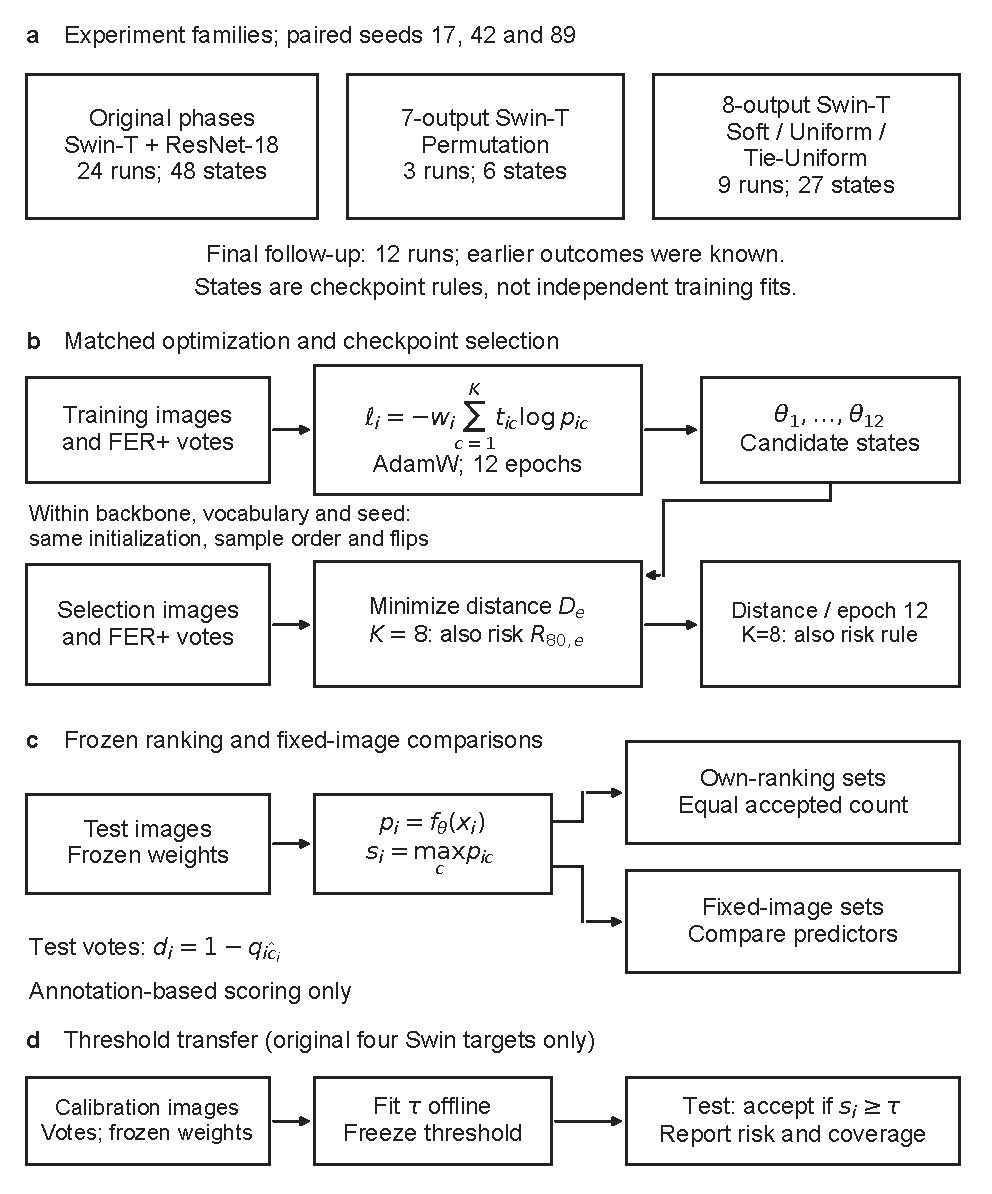
\includegraphics[width=\linewidth]{final_revision_2026_10_20/source/figures/StudyDesign.pdf}
\caption{Study design and adaptive follow-up. (a) Original experiments and the final twelve-run plan, frozen before its own outcomes after earlier findings were known. State counts identify checkpoint rules, not independent fits. (b) Matched training and selection: $D_e$ is selection-set complete-vocabulary squared distance; eight-output models additionally retain a separate state minimizing selection-set 80\% MSP disagreement $R_{80,e}$. Epoch 12 is retained independently. (c) Own-ranking fixes accepted counts; cross-evaluation fixes images. (d) Only the original Hard, Tie-hard, Uniform and Soft policy comparison fits calibration thresholds}\label{fig:design}
\end{figure}
\begin{figure}[!htbp]
\centering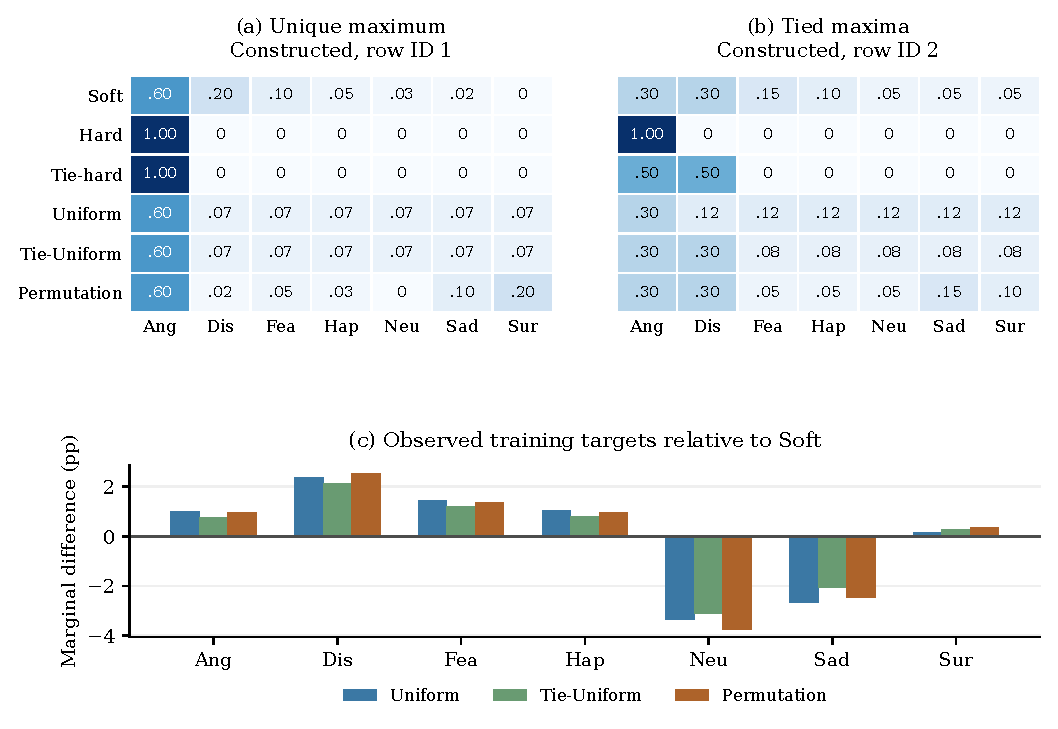
\includegraphics[width=\linewidth]{final_revision_2026_10_20/source/figures/TargetIntervention.pdf}
\caption{Training-target interventions. (a,b) Constructed seven-class examples, rounded to two decimals; nominal row IDs 1 and 2 fix the deterministic permutation and are not sampled images. Permutation preserves every maximum position and the probability multiset. (c) Actual Training targets: weighted class marginals $\sum_iw_it_{ic}/\sum_iw_i$ relative to Soft, in percentage points. Zero-mass rows contribute zero weight. Ang, Dis, Fea, Hap, Neu, Sad and Sur denote angry, disgust, fear, happy, neutral, sad and surprise. Equal per-image entropy need not preserve aggregate class proportions}\label{fig:targets}
\end{figure}

\subsection{Models, preprocessing and optimization}
Swin-T uses torchvision ImageNet-1K V1 initialization \cite{liu2021swin,deng2009imagenet,paszke2019pytorch}. One post-pooling channel gate transforms its 768-vector:
\begin{equation}
\tilde z=z\odot\sigma\!\left(W_2\operatorname{ReLU}(W_1z)\right),\quad
W_1\in\mathbb{R}^{48\times768},\ W_2\in\mathbb{R}^{768\times48}.
\end{equation}
The bias-free gate adds 73,728 parameters; a biased linear classifier gives the logits. ResNet-18 uses ImageNet-1K V1 features and a bias-free $512\to32\to512$ gate with 32,768 parameters \cite{he2016resnet}. The gate is fixed across target conditions and is not evaluated against an ungated model. Supplementary Fig.~S11 details the hierarchy.

Images are converted to grayscale, repeated across three channels, resized to $224\times224$ by bilinear interpolation and normalized with mean/std 0.5. The only augmentation is a horizontal flip determined by seed, epoch and original row. Seeds 17, 42 and 89 share initialization, sample order and flips across matched targets; classifiers are reset with Torch seed $1000+\mathrm{seed}$. Initial-state hashes verify matching within each output vocabulary. ResNet BatchNorm updates include zero-weight rows, which can affect its statistics.

All parameters train for 12 epochs with AdamW \cite{loshchilov2019adamw}: batch size 32, learning rate $10^{-4}$, weight decay $10^{-4}$, $\beta=(0.9,0.999)$ and $\epsilon=10^{-8}$. A cosine scheduler steps after each epoch with $T_{\max}=12$ and minimum $10^{-6}$. Training uses CUDA BF16 on an RTX 3070 Laptop GPU (8 GB), PyTorch 2.8.0+cu128 and torchvision 0.23.0+cu128. Deterministic algorithms control execution without promising identical results across platforms. This common budget is a matched comparison, not architecture-specific optimization or proof of convergence.

Selection minimizes mean ten-category squared distance after zero-padding model probabilities; ties retain the earlier epoch. Epoch 12 is evaluated independently. The criterion is common but not intrinsically neutral: the per-image Soft cross-entropy optimum is $p_c=q_c/w$, whereas the constrained squared-distance optimum is $p_c=q_c+(1-w)/K$ for $K$ supported outputs. They coincide at $w=1$. Retained fixed-epoch states test one alternative stopping decision; not all historical intermediate weights remain for reconstructing other selection criteria.

\subsection{Explanatory target and vocabulary follow-up}\label{sec:followup}
The final adaptive follow-up contains twelve new Swin-T runs: a seven-output minority-permutation target at seeds 17, 42 and 89, plus eight-output Soft, Uniform and Tie-Uniform at the same seeds. Training conditions, checkpoint rules and the primary analysis plan were frozen before full training, after the earlier manuscript and review findings were known. A separate ranking extension was frozen while training was underway, before any new calibration or test inference; original outcomes were already known. Every new epoch's weights and selection predictions are retained locally; all twelve runs finished and were hashed before new calibration or test inference. No condition was added or omitted according to its result.

The permutation target fixes every category position attaining the maximum. Remaining positions are cycled in a row-specific shuffled order, using PCG64 seeded from the SHA-256 digest of \texttt{minority-permutation-20261020:} and the original row ID. This mapping stays fixed across epochs and training seeds. It preserves each row's probability multiset, entropy and all maximum positions, while disrupting minority-category assignment when unequal values move. Rows with fewer than two nonmaximum positions are unchanged; duplicate probabilities can also yield an unchanged target. It changes 20,308 of 28,709 Training targets (70.74\%; 71.11\% of positive-mass rows). Its weighted class-marginal L1 difference from Soft is 0.1242 (Fig.~\ref{fig:targets}). Aggregate priors are therefore not preserved, limiting causal interpretation despite matching per-image entropy. Seven-output initialization is checked against the retained original runs.

The expanded vocabulary appends contempt as the eighth expression output; unknown and not-a-face remain outside the classifier and remain in the ten-category reference. Supported mass and targets are recomputed for $K=8$, leaving 150 zero-mass Training rows. Soft retains $r$, Uniform assigns $(1-m)/(K-1)$ off its chosen maximum, and Tie-Uniform assigns $(1-km)/(K-k)$ off its $k$ tied maxima when $k<K$. When all $K$ positions tie, Tie-Uniform assigns $1/K$ to each. Within each eight-output seed, targets share initialization, sample order, augmentation and the original twelve-epoch budget. The vocabulary comparison changes output dimension and supported weights together; it evaluates that policy change rather than a uniquely isolated contempt effect.

Distance-selected and epoch-12 states are reported for all new runs. A predeclared additional rule selects the earliest epoch minimizing complete-vote disagreement at 80\% MSP coverage on the selection subset for every eight-output condition. It tests a different stopping objective without choosing on test outcomes. This alternative cannot be reconstructed for all historical seven-output runs, whose intermediate weights were not retained.

The principal descriptive follow-up is distance-selected eight-output Soft minus Uniform at 80\% own-MSP coverage, with all three paired differences, sample standard deviation and conditional pixel-cluster intervals. The fixed epoch-12 comparison is a planned budget-matched sensitivity; the separately risk-selected comparison is an additional stopping sensitivity, not a replacement chosen for its test result. Tie-Uniform and permutation comparisons, full-coverage distance, fixed-set cross-evaluation, risk components and coverage curves are retained regardless of direction. These analyses extend the same exposed source rather than repair prior test reuse. Reported intervals condition on the fitted models and annotations and do not establish generalization over future training seeds.


\subsection{Disagreement and accepted-image comparisons}
For predicted class $\hat c_i$, disagreement with one draw from the observed annotations is $d_i=1-q_{i\hat c_i}$. Its available-class floor and excess are
\begin{equation}
b_i=1-\max_{c\leq K}q_{ic},\quad e_i=\max_{c\leq K}q_{ic}-q_{i\hat c_i},\quad d_i=b_i+e_i.
\label{eq:decomposition}
\end{equation}
Equivalently,
\begin{equation}
d_i=\underbrace{1-w_i}_{\text{unsupported mass}}+
\underbrace{w_i-\max_{c\leq K}q_{ic}}_{\text{supported ambiguity}}+e_i.
\label{eq:threeparts}
\end{equation}
This is accounting relative to finite observed votes, not a causal decomposition. Under ideal $p=r$, $d=1-w\max p$; thus MSP alone omits supported mass. For example, MSP 0.9 implies disagreement 0.1 at $w=1$ but 0.55 at $w=0.5$. Annotation-derived $w$ is unavailable at runtime and is not a selector.

The distributional endpoint is
\begin{equation}
D=\frac1N\sum_i\sum_{c=1}^{10}(\tilde p_{ic}-q_{ic})^2,
\end{equation}
where $\tilde p$ adds zeros for unsupported categories. It uses all 3,275 primary-test images and unmodified votes. Lower $D$ alone does not establish calibration. Weighted F1 is $\sum_c n_cF1_c/N$ against original FER2013 labels; crowd-majority F1 instead requires more than half of all votes for one supported category \cite{sokolova2009metrics}. Undefined class scores are zero. These references define different tasks.

At coverage $\gamma$, each model ranks by MSP and accepts $\lceil\gamma N\rceil$ rows, breaking ties by original row ID. The primary reporting point is $\gamma=0.8$; 0.2, 0.5, 1.0 and all-prefix curves provide sensitivity. Equal counts do not imply equal images. Cross-evaluation therefore scores each predictor on both selectors' fixed sets. Supported-mass strata distinguish $w=0$, $0<w<1$ and $w=1$; restricting a global accepted set differs from ranking separately within strata. The supplement reports both.

\subsection{Calibration, score sensitivity and uncertainty}
Empirical calibration selects the largest tie-preserving accepted set of at least 100 images whose observed disagreement is at most 10\%, 20\% or 30\%; otherwise it abstains completely. Thresholds are frozen for testing. A conservative comparator searches 101 fixed thresholds from zero to one and substitutes
\begin{equation}
U=\min\!\left(1,\bar d+\sqrt{\log(101/0.05)/(2n)}\right)
\end{equation}
for empirical risk. Hoeffding's inequality and a union bound motivate the margin for fixed models, independent identically distributed bounded losses and unchanged populations \cite{hoeffding1963}. Those deployment assumptions are unverified here. Empty accepted sets have undefined risk. One hundred shared pixel-cluster half-splits further describe within-calibration fit/holdout variation; overlapping resamples are not independent replications.

Within-source contrasts use 5,000 paired exact-pixel-cluster bootstrap replicates. The 3,275 test rows form 3,268 clusters: 3,261 singletons and seven pairs. Each replicate samples 3,268 clusters with replacement, applies common multiplicities to both conditions and all three seeds, reranks each model, and accepts $\lceil0.8N_b\rceil$ rows of its resampled image multiset of size $N_b$. It computes the three paired risk differences and averages them within that replicate. Percentile 95\% intervals therefore condition on the three fitted seed pairs and observed annotations. They exclude rater uncertainty, person-level dependence, variability over new training seeds and adaptive hypothesis selection. Secondary intervals are descriptive, without multiple-testing superiority claims; crossing zero does not establish equivalence.

Exploratory score analyses rank unchanged probabilities by MSP, top-two margin or negative entropy $\sum_cp_c\log p_c$ ($0\log0=0$). The full ledger includes all original 48 states and four coverages. Follow-up normalization and target-statistic diagnostics use the retained outputs under fixed reporting rules, with no test-based tuning of a new selector. Their methods and results appear with the follow-up analyses.

The separately frozen ranking extension covers all 33 new inference states and the six historical seven-output Soft states used as permutation comparators. These 39 named states are not independent fits. It reports MSP, margin, negative entropy, centered logit normalization and a calibration-only choice between MSP and normalization at 20\%, 50\%, 80\% and 100\% coverage. Each state's normalization exponent minimizes all-prefix mean calibration risk (AURC) over the ordered grid $1,1.5,2,3,4,6,8,16$; exact ties retain the first exponent. The two-score choice also uses calibration AURC, retaining MSP on ties; it does not choose among all five scores. All candidate test outcomes are retained but never select parameters. These descriptive ranking comparisons report paired-seed differences, sample standard deviations and ranges, without new bootstrap intervals. The extension was recorded during training before any new calibration or test inference, with the original results already known.

\subsection{External clips and retained-output diagnostics}\label{sec:external}
RAVDESS provides 1,440 video-only speech clips from 24 actors and ten original human category responses per clip \cite{livingstone2018ravdess}. Its S5 workbook includes the seven model expressions, calm and none. The original adult acted-video population differs from natural messaging faces. Original Zenodo media were obtained under CC BY-NC-SA 4.0 and are not redistributed.

All 36 original Soft, Uniform and Tie-Uniform states are transferred without fitting, peak selection or outcome filtering. Eight bin centers $\lfloor(b+0.5)N/8\rfloor$ are sampled, $b=0,\ldots,7$. A valid frame requires exactly one MediaPipe detection (model selection 1; confidence 0.5) and a clipped non-expanded crop; no fallback or manual repair is used. Shared preprocessing follows Sect.~3.4. At least four distinct valid frames are required. CUDA BF16 forward passes and float32 softmax produce frame probabilities, averaged in float64 before clip argmax. All 1,440 clips remain in the coverage denominator; insufficient eligibility makes an endpoint unavailable.

Raw scoring retains all nine responses. The required merged sensitivity adds calm to neutral while leaving none and predictions unchanged. Each model ranks clips by MSP, with filename-order ties. Actor uncertainty uses 5,000 paired samples of the 24 whole actors (RNG seed 11011); each replicate averages paired-seed differences after reranking its 1,440-clip multiset. Intervals condition on these fitted models, actors and votes. Exact $48\times48$ grayscale and 63-bit DCT crop hashes screen overlap against all 35,887 FER2013 images; perceptual distance at most four flags review, without establishing person separation.

\begin{figure}[!htbp]
\centering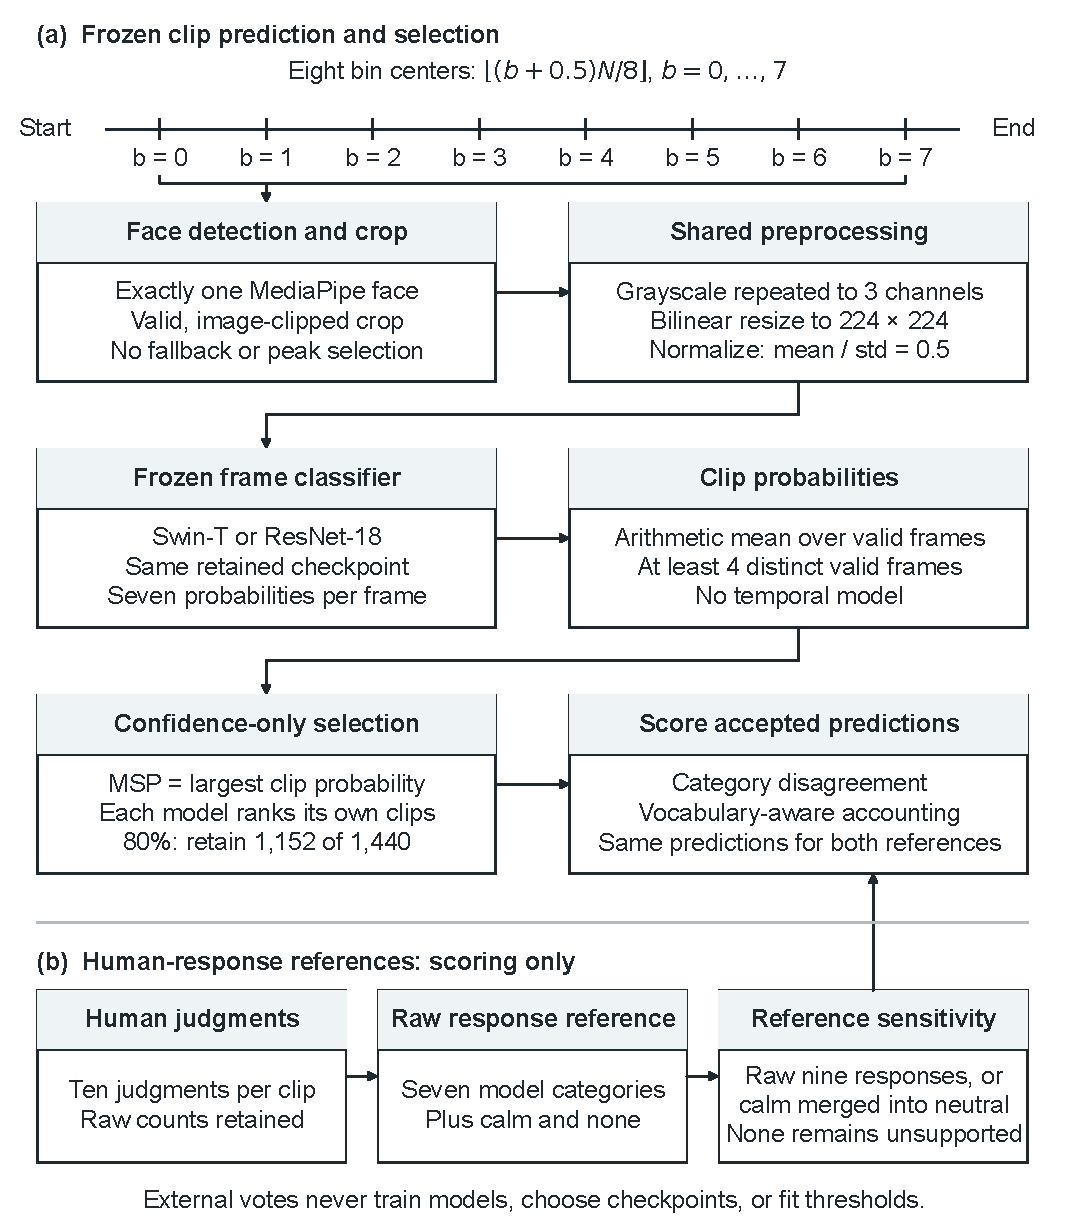
\includegraphics[width=\linewidth]{final_revision_2026_10_20/source/figures/ExternalPipeline.pdf}
\caption{Original frozen-model clip evaluation. Eight bin-center frames undergo fixed detection, cropping, preprocessing and inference. Valid-frame probabilities are averaged before clip prediction and confidence ranking. Every clip remains in the coverage denominator; votes enter scoring only. Raw and calm/neutral-merged references score unchanged outputs. Central-window aggregation is examined separately as a post hoc sensitivity}\label{fig:externalpipeline}
\end{figure}

Post hoc diagnostics retain class frequencies, every temporal bin and vote-weighted matrices $C_{ab}(A)=\sum_{i\in A}q_{ia}\mathbb I(\hat c_i=b)$. Row normalization uses accepted vote mass and is undefined for zero mass. These fractional contributions are not independent participant observations. Clip-level judgments do not establish frame accuracy. Follow-up constant-category references score all clips and the same model-fixed accepted sets; central-window aggregation tests a fixed alternative to eight-frame averaging. Both are exploratory, with no frame selection using outcomes.

\subsection{Local prototype and verification scope}
The supplementary Streamlit application is a local sender composition preview using MediaPipe \cite{lugaresi2019mediapipe}, the shared preprocessing, seven-class order and Swin head. The eight-output models are research comparisons and are not deployed in this preview. It has no recipient-side transport. Opt-in and invalid/stale-cue suppression are unvalidated design safeguards; offline calibration policies are not deployed in the app. Local processing requires the Python backend to run on the sender's machine. A categorical cue can itself be sensitive. Software checks verify numerical metrics, model contracts and failure handling, not communication effectiveness. AI assistance (OpenAI Codex) supported literature checks, code, drafting and technical verification; the authors remain responsible for the work.


\FloatBarrier
\section{Results}
\subsection{Original target and checkpoint comparisons}
At 80\% coverage, validation-selected seven-output Swin-T has mean complete-vote disagreement of 23.68\% for Soft and 24.06\% for Uniform (Table~\ref{tab:primary}). Soft minus Uniform is -0.38 percentage points (pp), with a conditional 95\% pixel-cluster interval of [-0.64, -0.07]. Each model accepts its own 2,620 images. The corresponding Soft-minus-Hard difference is -2.61 pp [-2.98, -2.19]; the substantially smaller matched-control difference changes the interpretation of that hard--soft comparison.
\begin{table}[!htbp]
\caption{Selected-checkpoint risk at 80\% coverage (2,620 of 3,275 images). Risk is mean $\pm$ sample SD; components are mean percentage points}\label{tab:primary}
\centering\begin{tabular}{lrrrr}\toprule
Targets & Risk (\%) & Unsupported & Ambiguity & Excess\\\midrule
Hard & $26.30 \pm 1.04$ & 6.65 & 16.14 & 3.51\\
Tie-hard & $25.82 \pm 0.58$ & 6.67 & 16.03 & 3.13\\
Uniform & $24.06 \pm 0.10$ & 6.41 & 15.41 & 2.24\\
Tie-Uniform & $24.27 \pm 0.17$ & 6.47 & 15.46 & 2.35\\
Soft & $23.68 \pm 0.07$ & 6.55 & 15.01 & 2.13\\
\bottomrule\end{tabular}\par
Accepted identities differ; components provide accounting, not causal attribution.
\end{table}


Tie-hard minus Hard is -0.47 pp [-0.80, -0.12], and Soft minus Tie-hard is -2.14 pp [-2.49, -1.76]. At fixed epoch 12, Soft minus Uniform remains negative (-0.32 pp [-0.63, -0.05]), whereas Soft minus Hard is -1.35 pp [-1.72, -1.05]. Soft also has lower disagreement than Tie-Uniform at both Swin checkpoint states. The supplement retains all seed differences, absolute risks, selected epochs, trajectories and coverage curves; these are correlated sensitivities on the same image source, not additional independent confirmations.

\subsection{Distributional agreement and backbone sensitivity}\label{sec:distance}
Soft has lower ten-category squared distance than Uniform and Tie-Uniform in every original seed, backbone and checkpoint state. For selected Swin-T, the means are 0.09783 versus 0.11571 and 0.11373 (Table~\ref{tab:distance}). This scores all 3,275 primary-test images, without rejection.
\begin{table}[!htbp]
\caption{Complete-vocabulary squared distances: means across three seeds on all 3,275 primary-test images. Values are unscaled distance units; lower is better}\label{tab:distance}
\centering\small\begin{tabular}{llrrr}\toprule
Backbone & State & Soft & Uniform & Tie-Uniform\\\midrule
Swin-T & Selected & 0.09783 & 0.11571 & 0.11373\\
Swin-T & Epoch 12 & 0.09779 & 0.11699 & 0.11280\\
ResNet-18 & Selected & 0.11059 & 0.12303 & 0.11805\\
ResNet-18 & Epoch 12 & 0.11089 & 0.12259 & 0.11665\\
\bottomrule\end{tabular}
\end{table}

The selective result is less consistent. Selected ResNet-18 gives Soft minus Uniform of +0.173 pp, compared with -0.378 pp for Swin-T; all four ResNet conditional intervals cross zero. Figure~\ref{fig:backbones} displays both outcomes with their distinct scales. Fixed-epoch values and all per-seed distributional scores appear in Supplementary Sect.~S2. These findings establish a difference between the measured outcomes for the tested models, without establishing a general architecture ordering.
\begin{figure}[!htbp]
\centering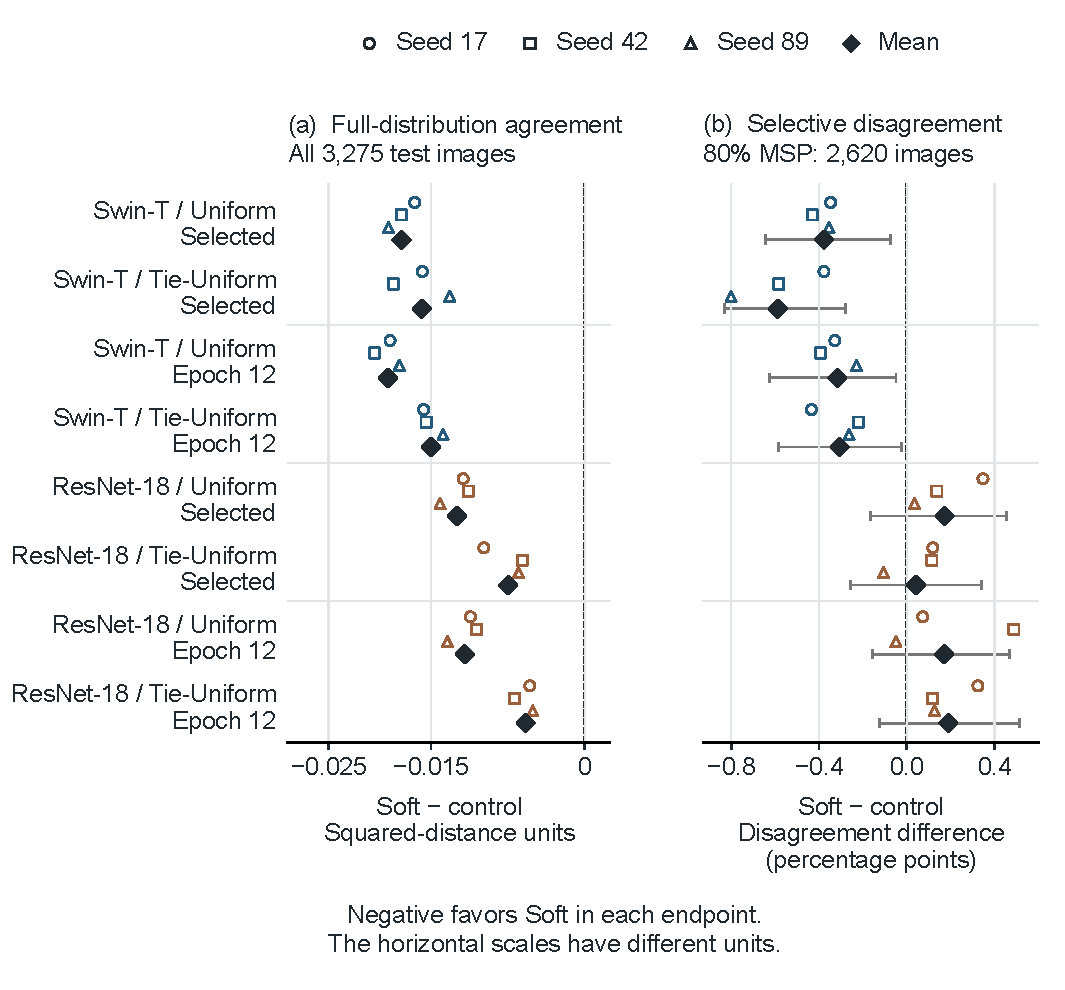
\includegraphics[width=\linewidth]{final_revision_2026_10_20/source/figures/Fig7.pdf}
\caption{Original Soft-minus-control differences. (a) Squared distance on all 3,275 images. (b) Complete-vote disagreement at 80\% own-ranking coverage. Symbols show three paired-seed contrasts and their mean; bars in (b) are conditional 95\% pixel-cluster intervals. No interval is shown in (a). The panels have different units and scales. Negative favors Soft}\label{fig:backbones}
\end{figure}

\subsection{Minority allocation and the eight-expression follow-up}\label{sec:new-results}
Preserving target probability values does not preserve the selective result. Distance-selected seven-output Soft has mean disagreement of 23.68\%, compared with 24.48\% for Permutation: a difference of $-0.794$ pp, with a conditional 95\% interval of $[-1.071,-0.474]$. The three paired differences are $-0.523$, $-0.935$ and $-0.924$ pp (sample SD 0.235 pp). At epoch 12, the mean remains negative ($-0.548$ pp, interval $[-0.855,-0.261]$). Thus, the observed minority allocation performs better than this particular entropy- and maximum-preserving permutation. The control changes aggregate class priors, so the comparison does not uniquely isolate category identity from those priors.

The principal eight-output comparison gives Soft 23.74\% disagreement, Uniform 24.58\% and Tie-Uniform 23.79\%. Soft minus Uniform is $-0.836$ pp, interval $[-1.152,-0.509]$, with paired differences $-0.454$, $-1.191$ and $-0.863$ pp (SD 0.369 pp). This contrast remains negative at epoch 12 ($-0.385$ pp) and under risk-based checkpoint selection ($-0.585$ pp). In contrast, Soft minus Tie-Uniform is only $-0.052$ pp, interval $[-0.314,+0.212]$. Its epoch-12 and risk-selected means are $-0.130$ and $-0.104$ pp, respectively; both intervals also cross zero. These intervals do not establish equivalence. Figure~\ref{fig:followup-contrasts} retains all eight planned contrasts, rather than only the larger differences against Uniform.

\begin{figure}[!htbp]
\centering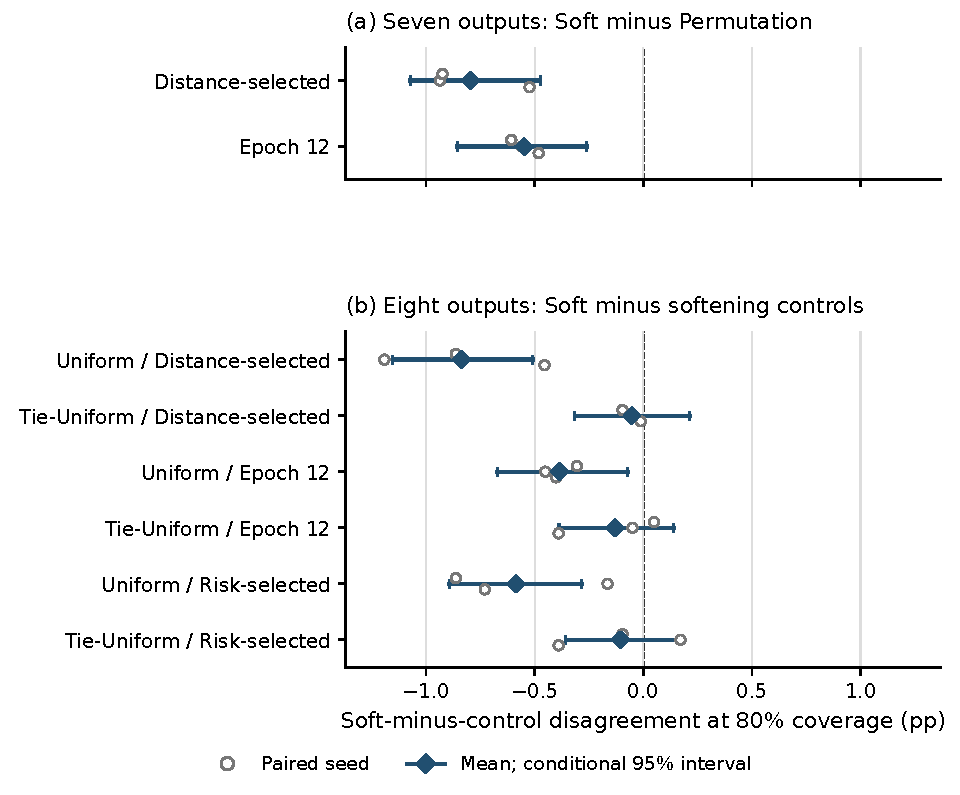
\includegraphics[width=\linewidth]{final_revision_2026_10_20/source/figures/FollowupContrasts.pdf}
\caption{Final adaptive follow-up at 80\% own-MSP coverage. Hollow symbols show three paired-seed differences, diamonds their mean, and bars conditional 95\% exact-pixel-cluster intervals. (a) Seven-output Soft minus Permutation. (b) Eight-output Soft minus Uniform or Tie-Uniform under all three checkpoint rules. Negative favors Soft. Distance selection is the principal rule; fixed epoch and risk selection are sensitivities. Different rules can select the same weights, and intervals do not represent uncertainty over new training seeds}\label{fig:followup-contrasts}
\end{figure}

Full-coverage distributional agreement remains more consistent. Eight-output Soft has lower ten-category squared distance than both softening controls in every seed and checkpoint rule. Distance-selected means are 0.09467 for Soft, 0.11708 for Uniform and 0.10962 for Tie-Uniform. However, expanding the vocabulary does not by itself establish a selective improvement: the seven- and eight-output Soft means are 23.68\% and 23.74\% on their separately accepted sets. This policy comparison changes supported weights, classifier dimension and fitted predictions together.

The new fixed-image comparisons also distinguish predictor changes from selection changes. For distance-selected eight-output models, Soft minus Uniform is $-0.729$ pp on Soft's accepted images and $-0.132$ pp on Uniform's images. Soft minus Tie-Uniform changes sign: $-0.279$ pp on Soft's images and $+0.125$ pp on Tie-Uniform's. The corresponding seven-output Soft-minus-Permutation means are $-0.523$ pp on Soft's set and $-0.074$ pp on Permutation's. These are means on identical images within each selector, not a causal decomposition of the own-ranking differences.

The separately frozen ranking extension reinforces the distinction. Calibration chose MSP over centered normalization for every new state, as it had for the original 48 states. For distance-selected eight-output Soft minus Tie-Uniform, the mean changes from $-0.052$ pp with MSP to $+0.280$ with margin, $+0.164$ with negative entropy and $+0.131$ with centered normalization. Predictions are unchanged; the accepted images change. Soft minus Uniform remains negative under these distance-selected scores, but its epoch-12 margin contrast is approximately zero ($+0.003$ pp). Supplementary Sect.~S11 retains every new state, seed, selected epoch, fixed-image comparison and ranking sensitivity. The findings support a conditional benefit against specific controls, not a score-independent advantage from retaining the full vote distribution.


\subsection{Identical images and annotation references}
Selected Swin-T's predictor ordering depends on who selects the images: Soft minus Uniform is +0.085 pp on Uniform-selected images but -0.352 pp on Soft-selected images (Fig.~\ref{fig:cross}). Within each set, the annotation reference and images are fixed, so the comparison concerns category choices. Changing from Uniform's set to Soft's set gives -0.025 pp for a fixed Uniform predictor and -0.463 pp for a fixed Soft predictor; mean Jaccard overlap is 0.8408. ResNet likewise changes sign between Uniform-selected (+0.445 pp) and Soft-selected images (-0.412 pp). The supplement retains both states and all seed matrices.
\begin{figure}[!htbp]
\centering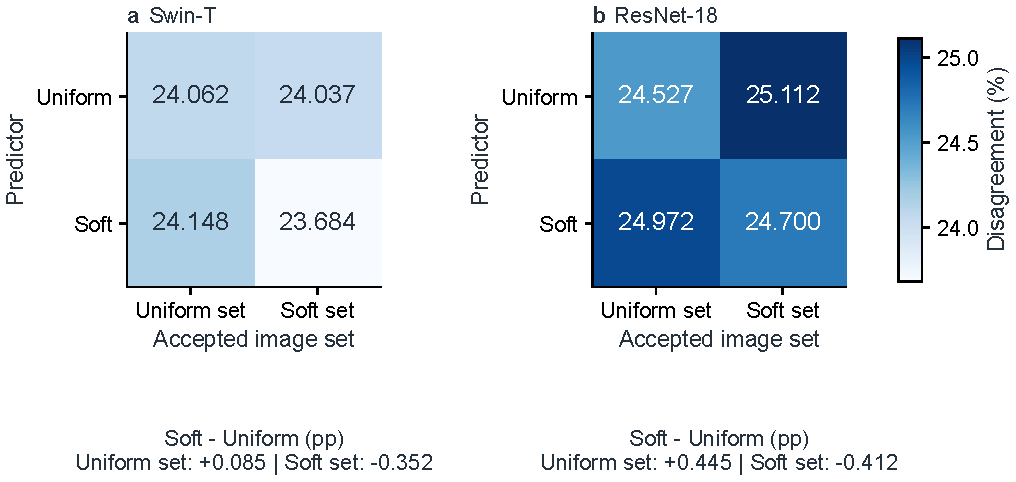
\includegraphics[width=\linewidth]{final_revision_2026_10_20/source/figures/Fig4.pdf}
\caption{Fixed-image cross-evaluation at 80\% coverage for selected (a) Swin-T and (b) ResNet-18. Cells show mean complete-vote disagreement (\%) across three seeds. Columns fix the selector's 2,620-image set; rows change the predictor. Signed Soft-minus-Uniform differences therefore hold images fixed. Each model's own-set risk uses different images}\label{fig:cross}
\end{figure}

The categorical reference also changes measured performance. On the same 2,484 supported-majority images, selected Swin-T Soft has weighted F1 0.6685 against original FER2013 labels and 0.9270 against crowd-majority labels. Against original labels, its score is 0.5722 on the full 3,275-image population. The first comparison changes the reference; the second changes the images. Neither changes the model predictions or establishes a new benchmark accuracy. Supplementary Sect.~S3 supplies complete same-image scores and the reference correspondence matrix.

\subsection{Unsupported categories and calibration transfer}
The original primary test set contains 1,732 fully supported, 1,527 partly supported and 16 zero-supported-mass images. At separately ranked 80\% within-stratum coverage, Soft/Uniform disagreement is 10.42\%/10.94\% for fully supported images and 40.00\%/40.58\% for partly supported images. The overall contrast is therefore not confined to images receiving unsupported votes. However, Soft accepts a mean 11.00 of the 16 zero-mass images, versus 7.00 for Uniform and 6.67 for Tie-Uniform. Lower overall disagreement does not imply better rejection of those inputs. Supplementary Sect.~S4 gives the global and within-stratum results, with contempt, unknown and not-a-face reported separately.

Empirical calibration fails to preserve its nominal targets: all 36 nonempty original test settings exceed them. These overlapping settings are not independent trials. At the 10\% target, Soft achieves 49.54\% coverage and 13.01\% risk, versus Hard's 38.35\% and 11.45\%. This is not an equal-achieved-risk coverage advantage.

The full-population annotation floor rises from 23.70\% in calibration to 26.67\% in testing, while unsupported mass rises from 5.72\% to 7.88\%. On Soft's accepted sets at the 20\% target, the +2.57 pp risk gap comprises +1.98 pp unsupported mass, +0.78 pp supported ambiguity and -0.19 pp excess (Fig.~\ref{fig:transfer}). These quantities describe rather than cause the gap. Calibration half-split holdout-minus-fit gaps average +0.05 to +0.19 pp, with broad descriptive 5th--95th-percentile ranges around -2.3 to +2.8 pp. The fixed-grid comparator yields 24 nonempty test settings with no overshoot, but fully abstains at the 10\% target for every condition and seed. Supplementary Sect.~S6 retains all thresholds, resamples and achieved risks.
\begin{figure}[!htbp]
\centering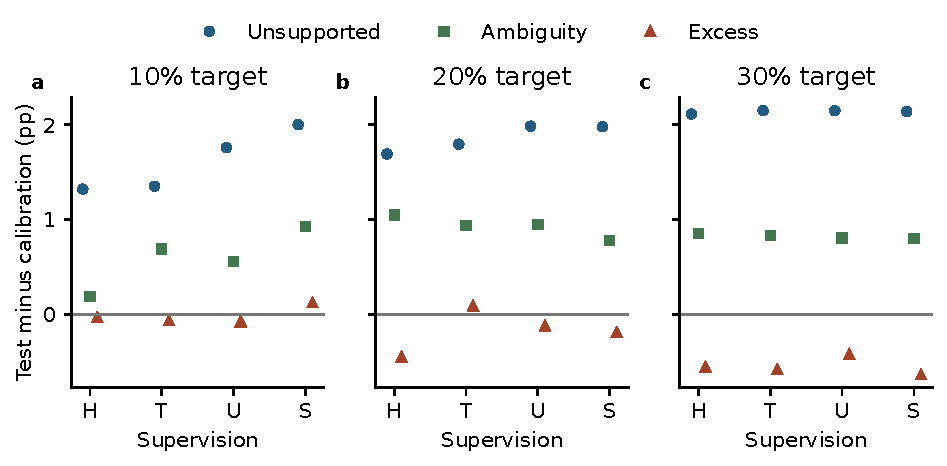
\includegraphics[width=\linewidth]{final_revision_2026_10_20/source/figures/Fig6.pdf}
\caption{Original calibration-to-test risk accounting. Mean differences in unsupported mass, supported ambiguity and excess sum to the risk gap on the respective accepted sets. H: Hard; T: Tie-hard; U: Uniform; S: Soft. Panels share a scale. These are descriptive components, not identified causes}\label{fig:transfer}
\end{figure}

\subsection{External clip transfer}
All 1,440 clips and 11,520 sampled frames meet the frozen rules, giving 100\% maximum coverage. At 80\% own-MSP coverage, selected Swin-T Soft has raw-reference disagreement of 68.37\%, Uniform 67.75\% and Tie-Uniform 67.42\%. Merging calm into neutral changes these to 60.72\%, 60.62\% and 60.03\%, while scoring the same predictions and accepted clips. This is agreement with human responses, not intended-expression accuracy.

The selected Swin Soft-minus-Uniform contrasts are -0.052, +2.639 and -0.755 pp for seeds 17, 42 and 89 under raw scoring: mean +0.611 pp, conditional actor interval [+0.23, +1.09]. Merged scoring gives -1.276, +2.483 and -0.903 pp: mean +0.101 pp [-0.26, +0.59]. Contrasts use unrounded risks. The positive mean is driven by seed 42 and does not establish a stable ordering over retraining. All three epoch-12 Swin contrasts favor Soft under merged scoring, illustrating checkpoint dependence. Figure~\ref{fig:external} and Supplementary Sect.~S7 retain both controls, backbones, states and references.
\begin{figure}[!htbp]
\centering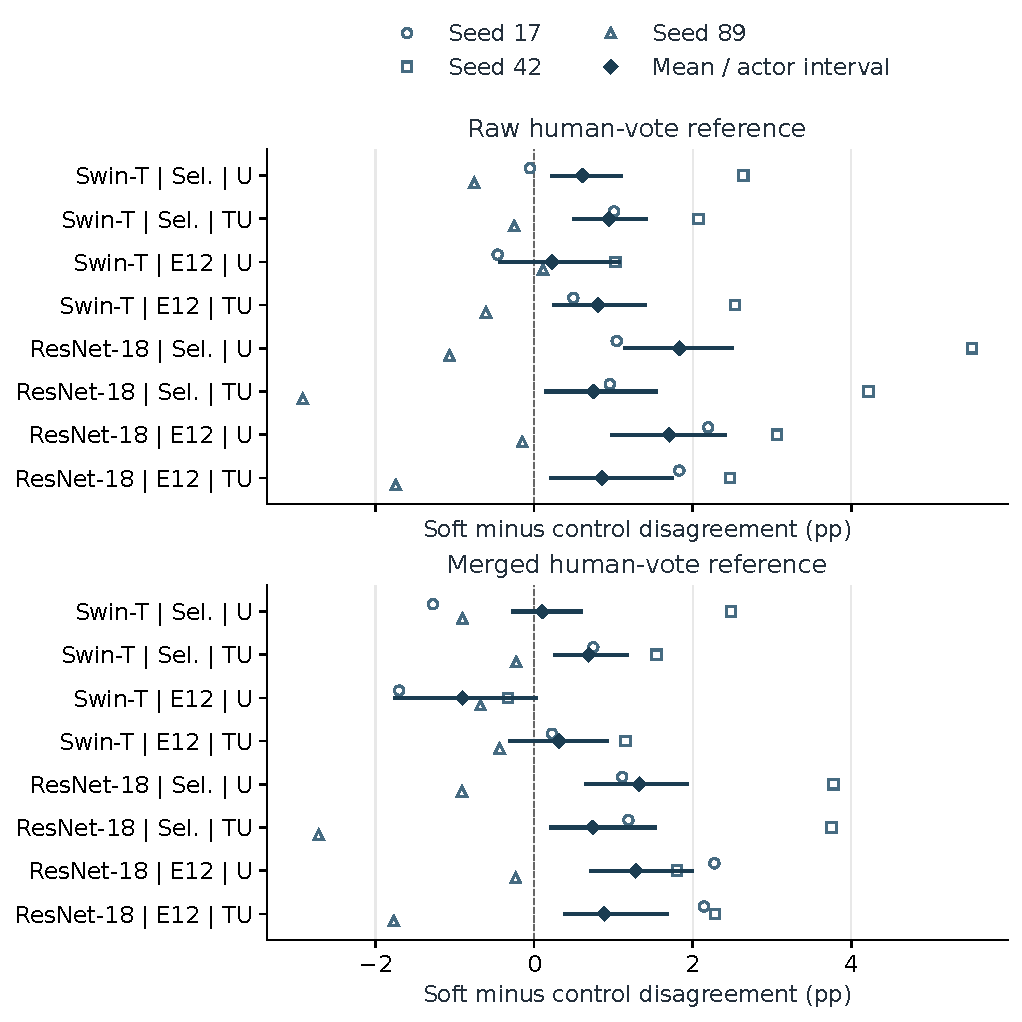
\includegraphics[width=\linewidth]{final_revision_2026_10_20/source/figures/ExternalContrasts.pdf}
\caption{Original external Soft-minus-control disagreement differences at 80\% own-MSP coverage. Hollow symbols show paired seeds; diamonds and bars show means and conditional 95\% actor-cluster intervals. Sel.: distance-selected; E12: epoch 12; U: Uniform; TU: Tie-Uniform. Negative favors Soft. The shared scale exposes seed variation; intervals condition on fitted pairs and observed actors/votes, not new seeds or raters}\label{fig:external}
\end{figure}

Transfer is poor for all conditions. Selected Swin Soft's raw all-clip risk is 71.06\%, comprising 11.90 pp unsupported mass, 16.81 pp supported ambiguity and 42.36 pp excess. On its accepted set, risk is 68.37\%, comprising 14.00, 16.61 and 37.76 pp, respectively. Thus, missing output categories alone cannot account for failure. Neutral comprises 67.0--70.0\% of accepted Soft predictions and 62.7--68.3\% of Uniform predictions. Vote-weighted matrices and eight-bin summaries describe these outputs, without treating clip labels as frame accuracy or assigning a cause to capture, population or aggregation. The follow-up aggregation and constant-category references below examine part of this interpretive uncertainty.

% Diagnostic exports follow the target, interpretation and transfer results.
\subsection{Exploratory checks of ranking, target entropy and temporal aggregation}
\label{sec:final-diagnostics}

These analyses use retained predictions after earlier outcomes were known. We applied the centered logit normalization studied by Xia et al.~\cite{xia2025smoothing}. For saved positive probabilities, let $z_c=\log p_c-K^{-1}\sum_j\log p_j$ and rank by $s_a=\max_c z_c/\lVert z\rVert_a$. The unknown softmax offset cancels, recovering centered logits algebraically; rounded float32 probabilities only approximate the original values. No saved probability required zero clipping. The exponent $a\in\{1,1.5,2,3,4,6,8,16\}$ minimizes mean all-prefix calibration risk (AURC) for complete-vote disagreement, with the first candidate resolving ties. Calibration selects parameters; test results remain exploratory. This adapts the published score to our endpoint rather than reproducing its original experiments.

Across all 48 original retained states, the best normalized score had worse calibration AURC than MSP. A calibration-only choice between MSP and normalization therefore retained MSP in every case. Normalization alone reduced the selected Swin-T Soft--Uniform advantage from $-0.378$ to $-0.223$ pp; ResNet-18 remained in the opposite direction (Table~\ref{tab:ranking-followup}). The small Swin-T contrast persists under this examined correction, although the calibration procedure selects MSP throughout. Class predictions remain unchanged, and full-coverage risk is score-invariant. These results concern crowd disagreement rather than the ordinary classification-error endpoint studied by Xia et al.

\begin{table}[!htbp]
\centering
\caption{Soft-minus-Uniform disagreement at 80\% coverage, in percentage points. Each score selects its own images. Centered normalization uses calibration-selected exponents; the calibration choice between scores equals MSP for all 48 original states. These are exploratory means over three fitted seed pairs.}
\label{tab:ranking-followup}
\begin{tabular}{llrr}
\toprule
Backbone & State & MSP & Centered norm \\
\midrule
Swin-T & selected & -0.378 & -0.223 \\
Swin-T & epoch12 & -0.317 & -0.122 \\
ResNet-18 & selected & +0.173 & +0.355 \\
ResNet-18 & epoch12 & +0.170 & +0.459 \\
\bottomrule
\end{tabular}

\end{table}

The controls also differ in measurable training-target properties. On the 28,557 positive-mass training images, mean entropy is 0.5067 nats for Soft, 0.8002 for Uniform and 0.7727 for Tie-Uniform. After weighting by supported vote mass, the corresponding values are 0.4949, 0.7812 and 0.7553. Their weighted class-marginal L1 differences from Soft are 0.1197 and 0.1032. These quantities substantiate the remaining entropy and class-proportion differences; they do not identify a causal minority-category mechanism. The 152 zero-mass images contribute no supervised target loss.

For all 36 external states, we compared the original eight-frame mean with the fixed middle four sampled positions (2--5, zero-based). Positions were determined chronologically within each clip before averaging; the window was not tuned against outcomes. We reranked all 1,440 clips separately under each aggregation and retained 1,152 at 80\% coverage. Reconstructing the original eight-frame means exactly matched every stored clip probability vector. For selected Swin-T Soft, the middle window reduced mean raw-reference disagreement from 68.37\% to 63.84\%, and calm-merged disagreement from 60.72\% to 56.71\% (Fig.~\ref{fig:aggregation-followup}). Its neutral prediction fraction decreased from 68.37\% to 55.09\%. The raw Soft--Uniform contrast remained positive ($+0.61$ versus $+0.59$ pp); the calm-merged contrast changed from $+0.10$ to $-0.21$ pp with mixed seed directions. Temporal aggregation affects absolute transfer performance substantially without establishing a stable supervision advantage.

\begin{figure}[!htbp]
\centering
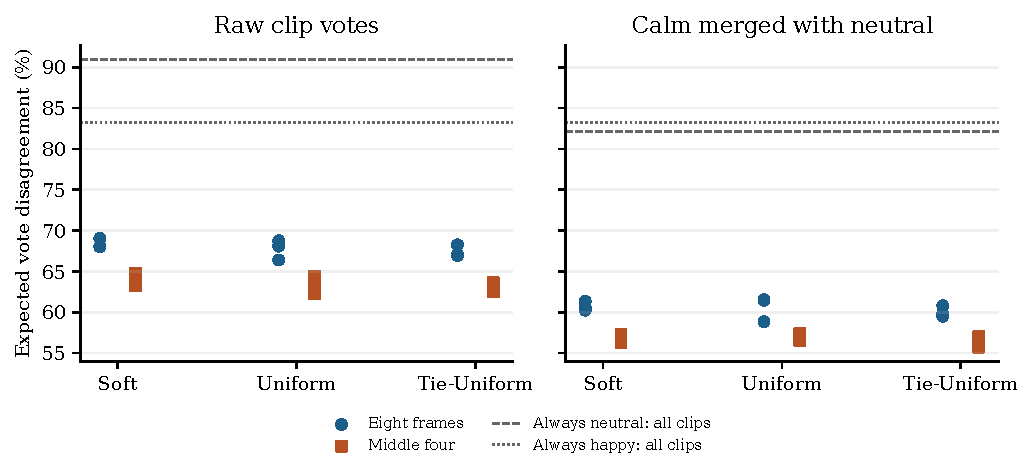
\includegraphics[width=\linewidth]{final_revision_2026_10_20/source/figures/ExternalAggregation.pdf}
\caption{Exploratory temporal aggregation for validation-selected Swin-T. Points show three seeds at 80\% coverage under each model's own MSP ranking. Reference lines show constant-category predictions on all 1,440 clips, a different population from the selected points. Exact accepted-set references are reported separately. The middle window is fixed, and clip-level human votes provide no frame-level ground truth.}
\label{fig:aggregation-followup}
\end{figure}

Always predicting neutral gives 90.94\% disagreement on all clips under raw scoring and 82.18\% after merging calm; always predicting happy gives 83.23\% under either reference. On the exact accepted sets of the original selected Swin-T Soft models, always-neutral risks average 88.80\% raw and 78.12\% merged; always-happy risk is 79.45\% under both references. The models outperform these simple references but still transfer poorly. Constants have no confidence ranking. Per-seed values, both backbones and states, exact-set references and calculation audits accompany the release. The checks narrow possible explanations without identifying a unique cause or establishing communication benefit.


\section{Discussion}
The general distinction between matching human response distributions and predicting their categories is established in FER and subjective language tasks \cite{barsoum2016ferplus,washington2021crowdsourcing,khurana2024crowd}. Our contribution is an empirical account of how specified target changes, output vocabulary and accepted images affect that distinction. The original Swin hard--soft difference falls from 2.61 pp to 0.38 pp against Uniform and does not persist in the ResNet comparison. The entropy-preserving permutation adds evidence that target probability values alone do not explain the observed ordering, although its changed class priors prevent a unique category-identity interpretation.

The eight-output results make the control dependence clearer. The distance-selected difference is 0.84 pp against Uniform but only 0.05 pp against Tie-Uniform; the latter changes direction under other confidence scores. Multiplying these own-ranking differences by 2,620 gives approximately 21.9 and 1.4 expected annotation-draw disagreements, respectively. These are count differences between separately selected populations, not the number of identical images corrected. The near-zero Tie-Uniform contrast does not prove equivalence, but it limits claims that detailed minority proportions generally improve selective decisions beyond preserving ties and dominant probabilities.

Identical-image comparisons add information that the own-ranking mean cannot supply. The predictor ordering changes with the selector's accepted set, so a lower selective risk does not establish uniformly better category choices on a fixed population. This pattern motivates reporting cross-evaluation alongside coverage curves; it does not identify a unique causal contribution of predictor versus selector. Likewise, the unsupported-mass decomposition is an algebraic identity. Its empirical role is to reveal how much of observed disagreement lies outside the available outputs and how that composition changes between accepted populations, not to establish a new theorem or diagnose internal emotion.

The follow-up target, vocabulary and ranking comparisons address explanations left open by the original results. Adding contempt changes supported weights and classifier dimension together and does not lower Soft's own-ranking risk in this comparison. The alternative stopping rule retains a Soft--Uniform advantage but does not resolve a consistent Soft--Tie-Uniform advantage. Lower squared distance across the matched conditions is partly expected from objective alignment; its value here is that it contrasts with the less stable categorical ordering, not that it establishes a new learning principle.

The external and calibration findings limit practical interpretation. Transferred empirical thresholds overshoot, and the conservative comparator sacrifices coverage. RAVDESS results are sensitive to checkpoint, seed and reference and exhibit substantial category-choice excess. Aggregation sensitivity can locate one pipeline dependence but cannot separate all effects of source population, cropping context and capture conditions. Confidence ranking is also a plausible explanation in light of label-smoothing results \cite{xia2025smoothing}; distributional distance alone cannot certify a useful rejector or calibrated risk \cite{baan2022calibration,guo2017calibration}. The supplementary preview consequently remains outside the validated operational scope.

\subsection{Limitations}
All training phases adaptively reuse FER2013 images with FER+ annotations. The final follow-up and locally frozen external plan preserve their timing records but do not restore an untouched static-image evaluation. Exact-pixel isolation and perceptual screening address particular overlap routes; identities and near-duplicate independence remain unverified. Conditional intervals describe resampling the observed pixels or actors for the retained fits. They omit uncertainty over raters, new seeds and populations and do not compensate for prior hypothesis selection.

Three paired seeds, two backbones and a fixed twelve-epoch recipe provide limited optimization evidence. The new eight-output stopping sensitivity tests an additional selection objective, not all schedules or hyperparameters. Vocabulary expansion and permutation address specified explanations rather than every effect of entropy, priors or regularization. Human vote frequencies are finite-panel observations, not emotion truth. RAVDESS is adult acted speech video with clip judgments, not a naturalistic messaging sample or independent static-image training replication.

No communication, demographic, cultural or mobile-efficiency study is supplied. Detector failures, pose, lighting and accessories may affect the local preview, whose update/freshness controls have not been validated through user research. Historical preprint manual-curation scores remain excluded because their records and checkpoints were not retained. These scope limits restrict generalization; they do not justify favourable unobserved results.


\section{Conclusion}
This adaptive study distinguishes distributional agreement from selective category disagreement through matched targets, fixed-image comparisons and complete-vocabulary scoring. Seven-output Soft outperforms the tested minority permutation despite matched per-image entropy and maxima. With eight outputs, its advantage persists against Uniform but is small and ranking-dependent against Tie-Uniform. Distributional agreement is more consistent than these selective differences; the backbone and external comparisons further limit generalization. The results support evaluating crowd supervision against explicit controls and reporting which images and annotation categories each outcome covers. They do not establish universal superiority of full-distribution training, a new architecture, or validated messaging benefits.


\backmatter
\section*{Statements and Declarations}
\noindent\textbf{Funding.} No funds, grants, or other support were received for preparation of this manuscript.

\noindent\textbf{Competing interests.} The authors declare no competing interests.

\noindent\textbf{Author contributions.} Gunjan Kumar Mishra conceived the prototype and led manuscript preparation. Bijaya Ghimire contributed to implementation, experimental design, and manuscript revision. Badri Raj Lamichhane supervised the work, contributed to methodology review, interpretation, and manuscript revision, and serves as corresponding author. Alan Shah contributed to literature review and code testing. All four authors confirmed the authorship arrangement and declarations.

\noindent\textbf{Ethics approval.} This study comprises secondary analysis of existing benchmark images, video-only speech clips and annotations, together with software tests. No institutional ethics approval or exemption determination was obtained.

\noindent\textbf{Consent to participate.} No participants were recruited and no new human ratings were collected. The RAVDESS publication reports consent and ethics review for its original collection; this does not constitute approval of this analysis. Photograph-level FER consent records were not independently verified.

\noindent\textbf{Consent for publication.} No identifiable facial photograph is reproduced. Interface illustrations contain synthetic text and no participant images.

\noindent\textbf{Data availability.} FER2013 acquisition records \cite{goodfellow2013fer}, official FER+ annotations \cite{barsoum2016ferplus}, hashes, role assignments and sample-level probabilities accompany the release. Complete ten-category annotations remain available for metric auditing. Original RAVDESS media and S5 human responses are available through its primary publication and Zenodo record \cite{livingstone2018ravdess}; derived counts and probabilities accompany the external diagnostics. Facial images and video are not redistributed.

\noindent\textbf{Code availability.} Versioned code, retained predictions, inference states and reproduction instructions are provided at \url{https://github.com/mgunjan67/crowd-supervision-selective-fer/releases/tag/v1.3.0}. The resource index maps each archive to its checksum and replay commands. The release covers 48 original and 33 new named checkpoint-rule states, which need not be distinct weights. All 144 new epoch weights remain locally retained; their hashes and selection outputs accompany the release, but intermediate epoch weights are not redistributed. The source ZIP separately compiles the current article and supplement. Numerical replay is internal verification, not external replication.

\noindent\textbf{Preprint statement.} An earlier version appeared on TechRxiv as ``Typing with Emotions: Facial Expression Recognition and Embedding in Text Messages,'' version 1, \url{https://doi.org/10.36227/techrxiv.175416003.30236370/v1}. This revision excludes participant evidence and unverifiable historical performance claims, corrects implementation descriptions and supplies documented new experiments. It does not claim to reproduce historical manual curation.

\noindent\textbf{Supplementary information.} The accompanying supplement contains per-seed outcomes, learning curves, fixed-image matrices, vocabulary and calibration diagnostics, external score/reference sensitivities, prototype details and provenance. The resource index maps each evidence archive and checkpoint collection to its checksum manifest and instructions.

\FloatBarrier
\bibliography{final_revision_2026_10_20/source/references}
\end{document}
